%========================================================
% Experiment 1 — Effective Fiber Models and BBM92 Performance
%========================================================

\subsection{Objective and Numerical Setup}

The first numerical experiment compares the effective fiber models introduced in
Chapter~\ref{ch:02_fiber_channel_modeling} from both a state-characterization
and an operational BBM92 perspective. The objective is to distinguish changes in
the quality of the distributed entangled state from changes in the correlations
observed in the fixed protocol measurement bases.

The input state is \(|\Psi+\rangle\) and three mechanisms are considered: coherent relative-phase evolution, statistical
dephasing, and symmetric local depolarization. For each propagated state, the
purity \(\gamma\), fidelity \(F\), concurrence \(C\), and basis-dependent error
rates \(Q_Z\) and \(Q_X\) are evaluated.

The operational classification is based on

\begin{equation}
Q_{\mathrm{worst}}
=
\max\left(Q_Z,Q_X\right),
\qquad
Q_{\mathrm{worst}}<Q_{\mathrm{th}},
\label{eq:exp1_operating_condition}
\end{equation}

with the threshold adopted in the present numerical analysis set to

\begin{equation}
Q_{\mathrm{th}}=0.11.
\label{eq:exp1_qber_threshold}
\end{equation}

The coherent-phase model is evaluated over \(181\) values of
\(\theta\in[0,\pi]\), while \(101\) points are used for both the dephasing and
depolarization sweeps.

%--------------------------------------------------------
% Coherent relative-phase evolution
%--------------------------------------------------------

\subsection{Coherent Relative-Phase Evolution}

A local relative phase produces the state

\begin{equation}
|\psi(\theta)\rangle
=
\frac{
|01\rangle
+
e^{i\theta}|10\rangle
}{
\sqrt{2}
}.
\nonumber
\label{eq:exp1_phase_state}
\end{equation}

Since this evolution is local and unitary, purity and concurrence remain equal
to unity. The fidelity with the initial Bell state and the BBM92 error rates are

\begin{equation}
F
=
\frac{1+\cos\theta}{2},
\qquad
Q_Z=0,
\qquad
Q_X
=
\frac{1-\cos\theta}{2}.
\label{eq:exp1_phase_results}
\end{equation}

The numerical results in Figure~\ref{fig:exp1_coherent_phase} reproduce this
behavior. In particular, the state remains maximally entangled while the error
rate in the diagonal basis increases with the uncompensated relative phase.

\begin{figure}[htbp]

    \centering

    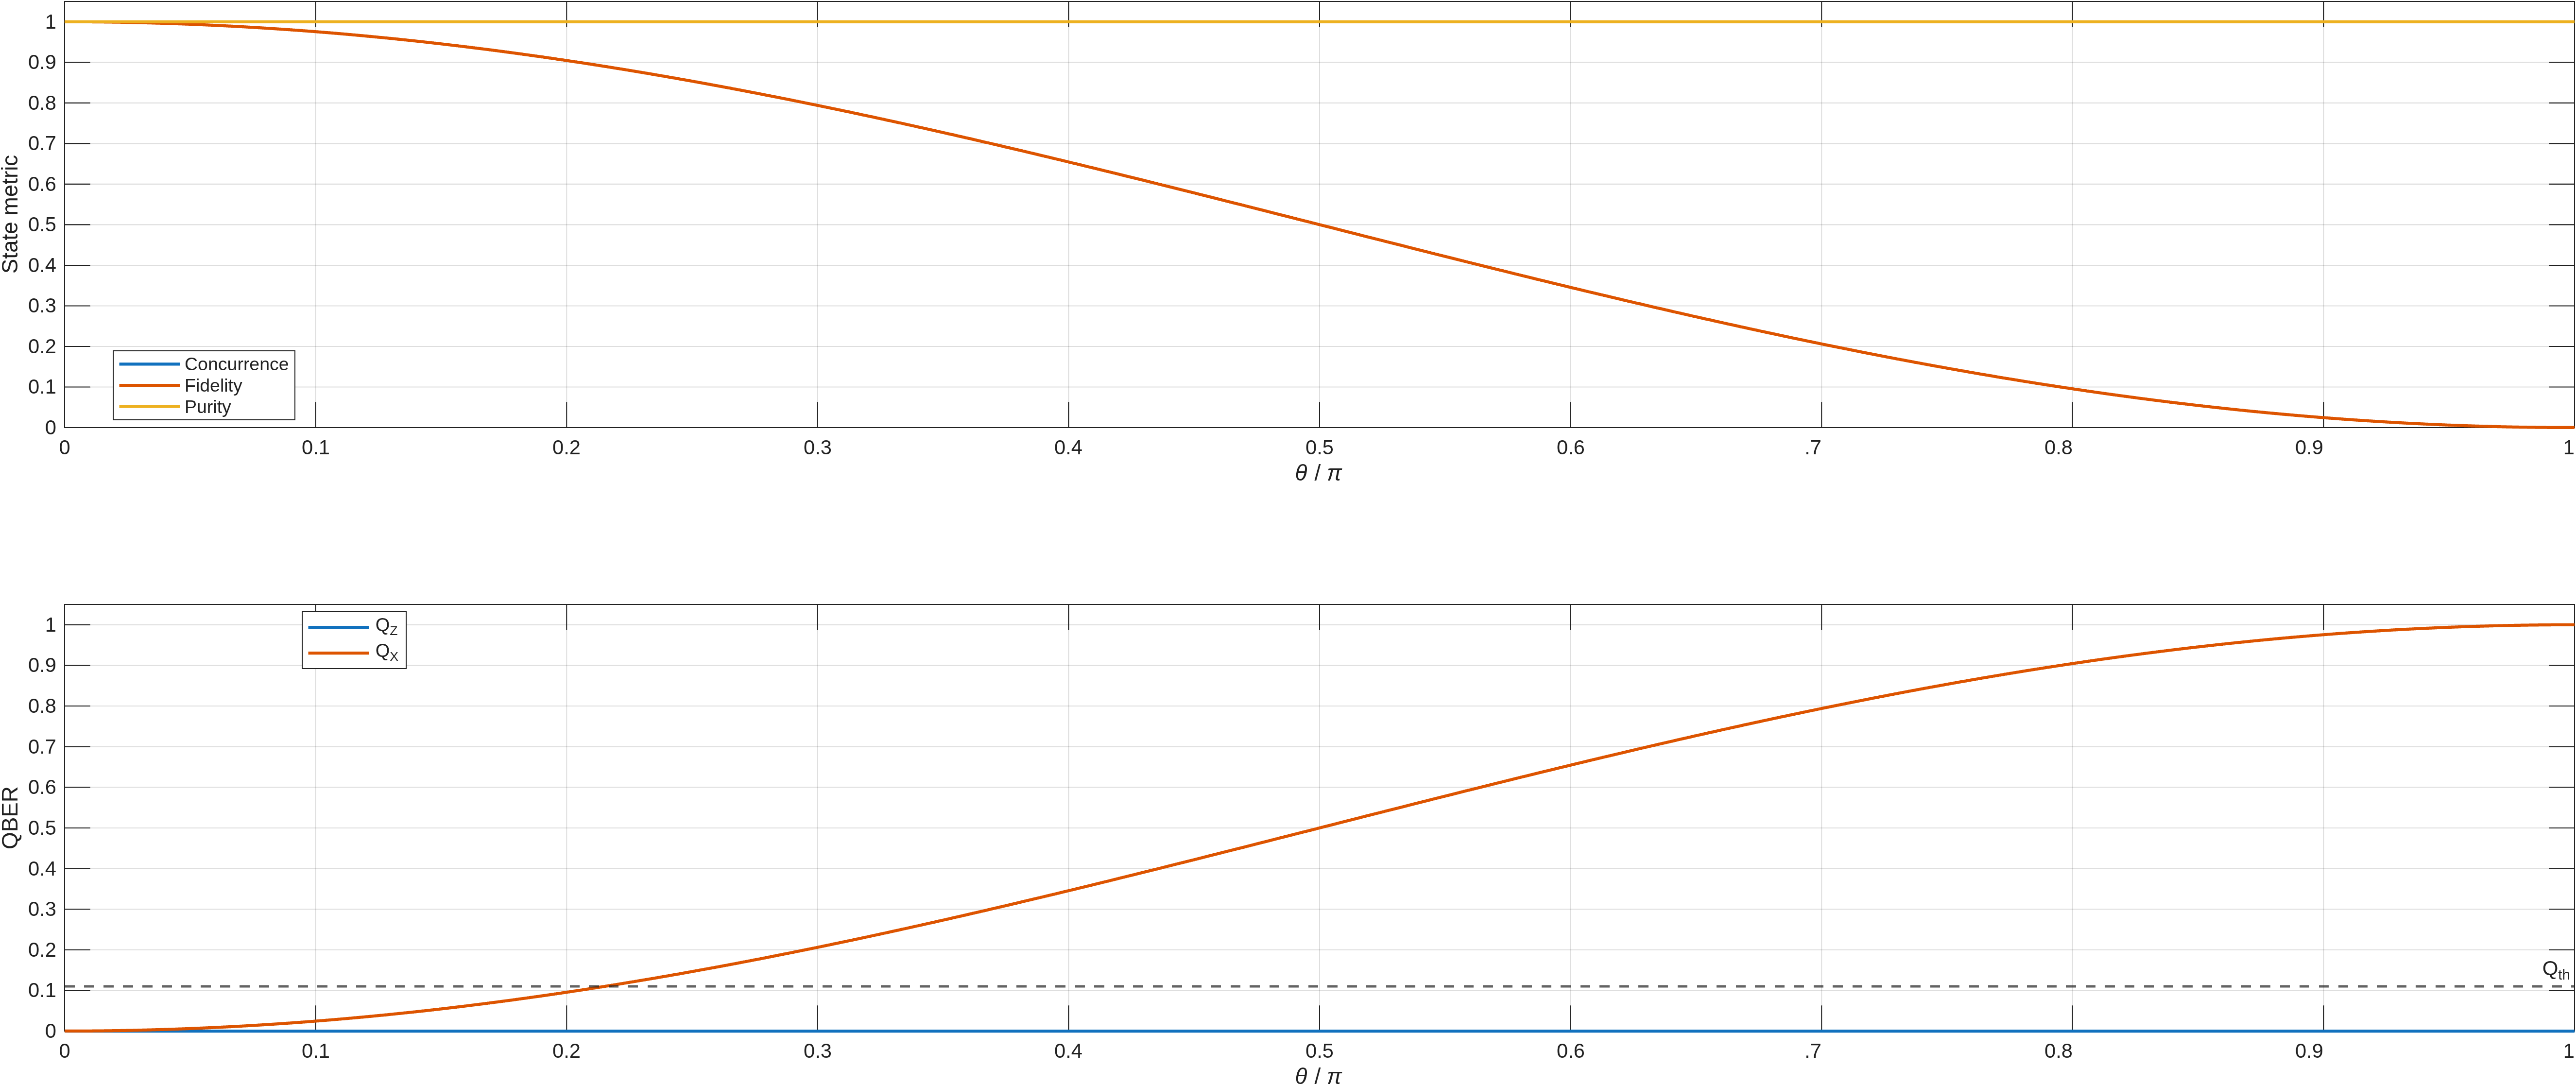
\includegraphics[
        width=0.98\textwidth
    ]{
        figures/experiment_1/phase_summary.png
    }

    \caption{
        Coherent relative-phase evolution. Purity and concurrence remain equal
        to unity, while fidelity and the diagonal-basis QBER vary with the
        relative phase. The dashed line indicates the adopted BBM92 QBER
        threshold.
    }

    \label{fig:exp1_coherent_phase}

\end{figure}

The corresponding numerical operating boundary is

\begin{equation}
\theta_{\mathrm{th}}
\simeq
0.6761~\mathrm{rad}
\simeq
0.215\pi.
\label{eq:exp1_phase_boundary}
\end{equation}

This case directly demonstrates that maximal entanglement does not by itself
guarantee low QBER when measurements are performed in fixed polarization bases.


%--------------------------------------------------------
% Statistical dephasing
%--------------------------------------------------------

\subsection{Statistical Dephasing}

Statistical fluctuations of the relative phase reduce the polarization
coherence. For the real coherence parameter \(\mu\in[0,1]\), the resulting state
is

\begin{equation}
\rho_{\mu}
=
\frac{1}{2}
\left(
|01\rangle\langle 01|
+
|10\rangle\langle 10|
\right)
+
\frac{\mu}{2}
\left(
|01\rangle\langle 10|
+
|10\rangle\langle 01|
\right).
\label{eq:exp1_dephasing_state}
\end{equation}

For this state family,

\begin{equation}
C=\mu,
\qquad
Q_Z=0,
\qquad
Q_X=\frac{1-\mu}{2}.
\label{eq:exp1_dephasing_results}
\end{equation}

As shown in Figure~\ref{fig:exp1_dephasing}, decreasing coherence now corresponds
to genuine entanglement degradation and increasing error in the diagonal basis.

\begin{figure}[htbp]

    \centering

    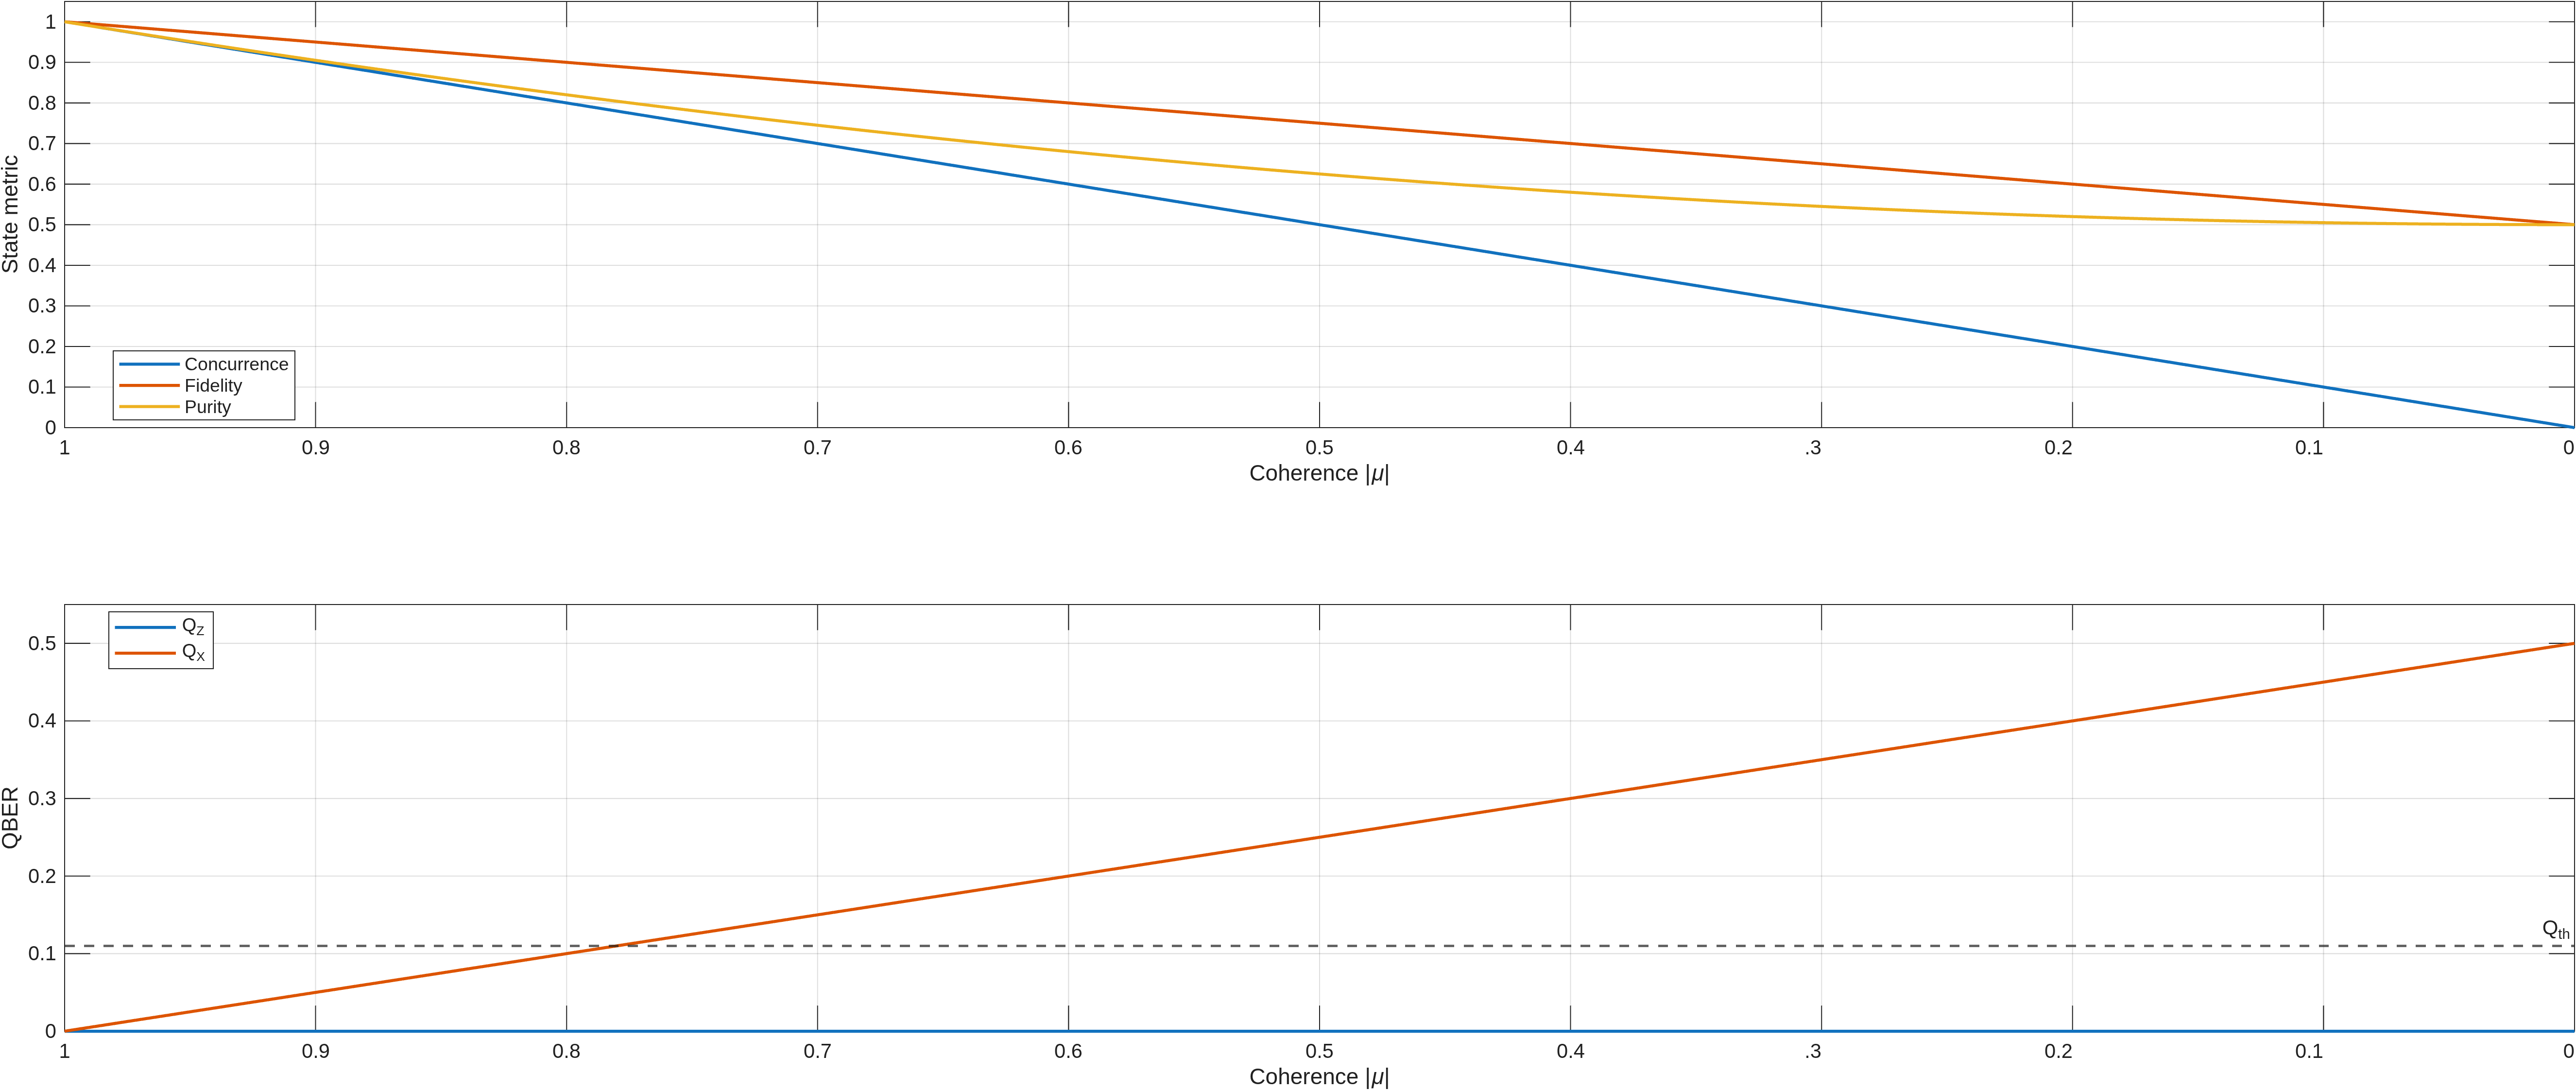
\includegraphics[
        width=0.98\textwidth
    ]{
        figures/experiment_1/dephasing_summary.png
    }

    \caption{
        Statistical dephasing as a function of the coherence parameter
        \(\mu\). Loss of coherence reduces concurrence, purity, and fidelity
        while increasing \(Q_X\); the \(H/V\)-basis correlations remain
        unaffected.
    }

    \label{fig:exp1_dephasing}

\end{figure}

The QBER threshold is crossed at

\begin{equation}
\mu_{\mathrm{th}}
=
0.780.
\label{eq:exp1_dephasing_boundary}
\end{equation}

Because \(C=\mu\) for this particular family, the same point corresponds to
\(C=0.78\). This value is specific to the dephasing model and does not represent
a universal concurrence threshold for BBM92 operation.


%--------------------------------------------------------
% Symmetric local depolarization
%--------------------------------------------------------

\subsection{Symmetric Two-Arm Depolarization}

The third model applies the same local depolarization probability to both
photons,

\begin{equation}
p_A=p_B=p.
\label{eq:exp1_symmetric_depolarization}
\end{equation}

In this case both measurement bases are affected. As shown in
Figure~\ref{fig:exp1_depolarization}, increasing \(p\) progressively decreases
purity, fidelity, and concurrence, while \(Q_Z\) and \(Q_X\) increase together.

\begin{figure}[htbp]

    \centering

    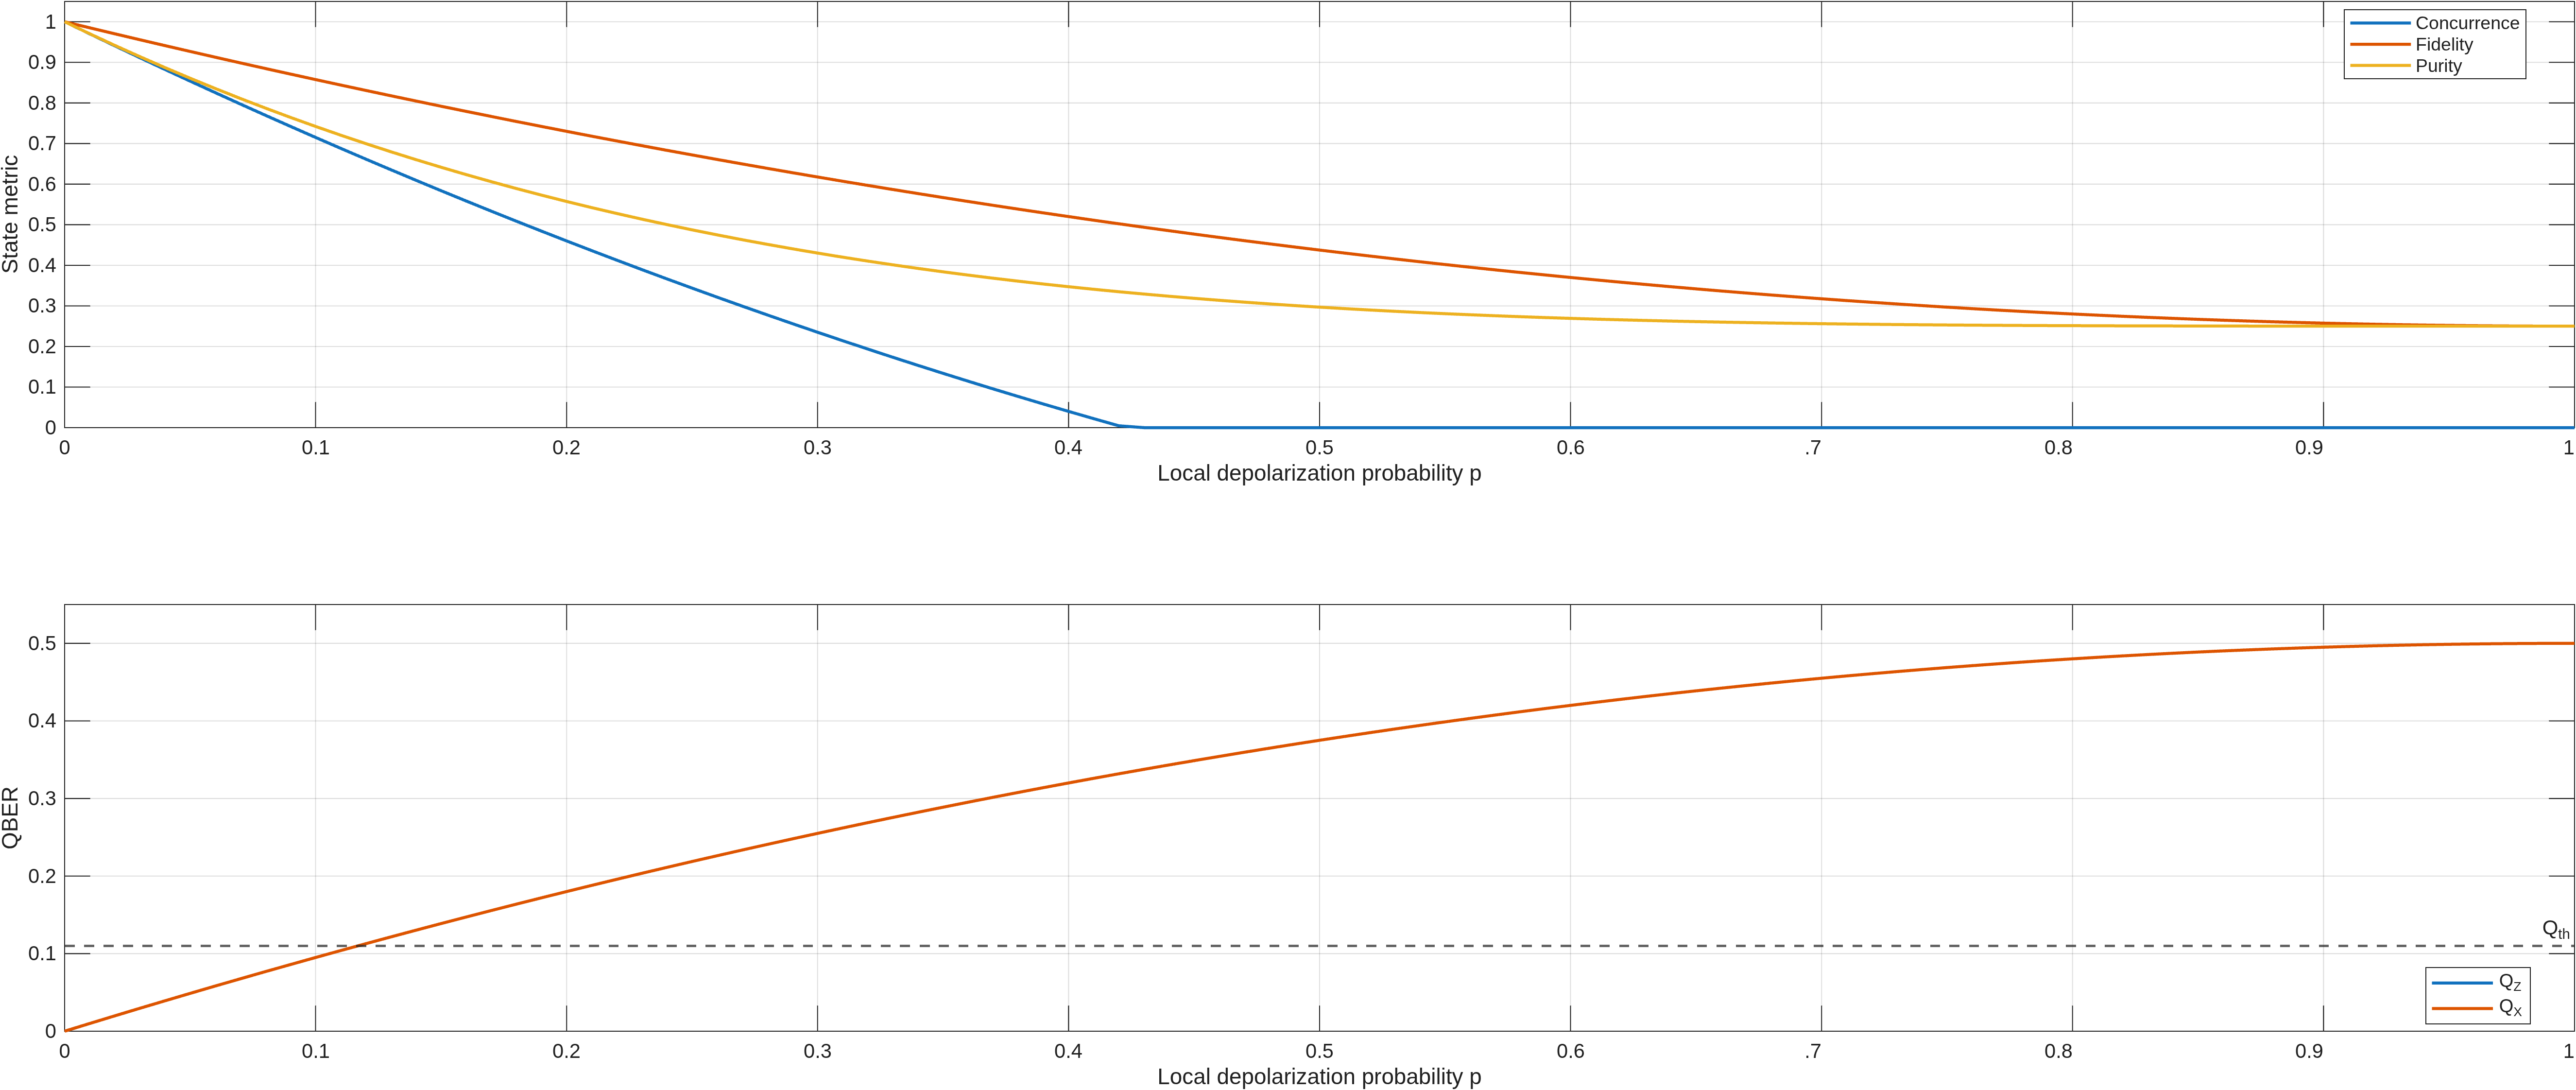
\includegraphics[
        width=0.98\textwidth
    ]{
        figures/experiment_1/depolarization_summary.png
    }

    \caption{
        Symmetric independent local depolarization. Increasing the local
        depolarization probability reduces the state-quality metrics and
        produces equal errors in the two BBM92 measurement bases.
    }

    \label{fig:exp1_depolarization}

\end{figure}

The numerical operating boundary is

\begin{equation}
p_{\mathrm{th}}
\simeq
0.1168.
\label{eq:exp1_depolarization_boundary}
\end{equation}


%--------------------------------------------------------
% Comparison
%--------------------------------------------------------

\subsection{Comparison of State Quality and BBM92 Performance}

Figure~\ref{fig:exp1_concurrence_qber} directly compares the worst-basis QBER
with concurrence for the three models.

\begin{figure}[htbp]

    \centering

    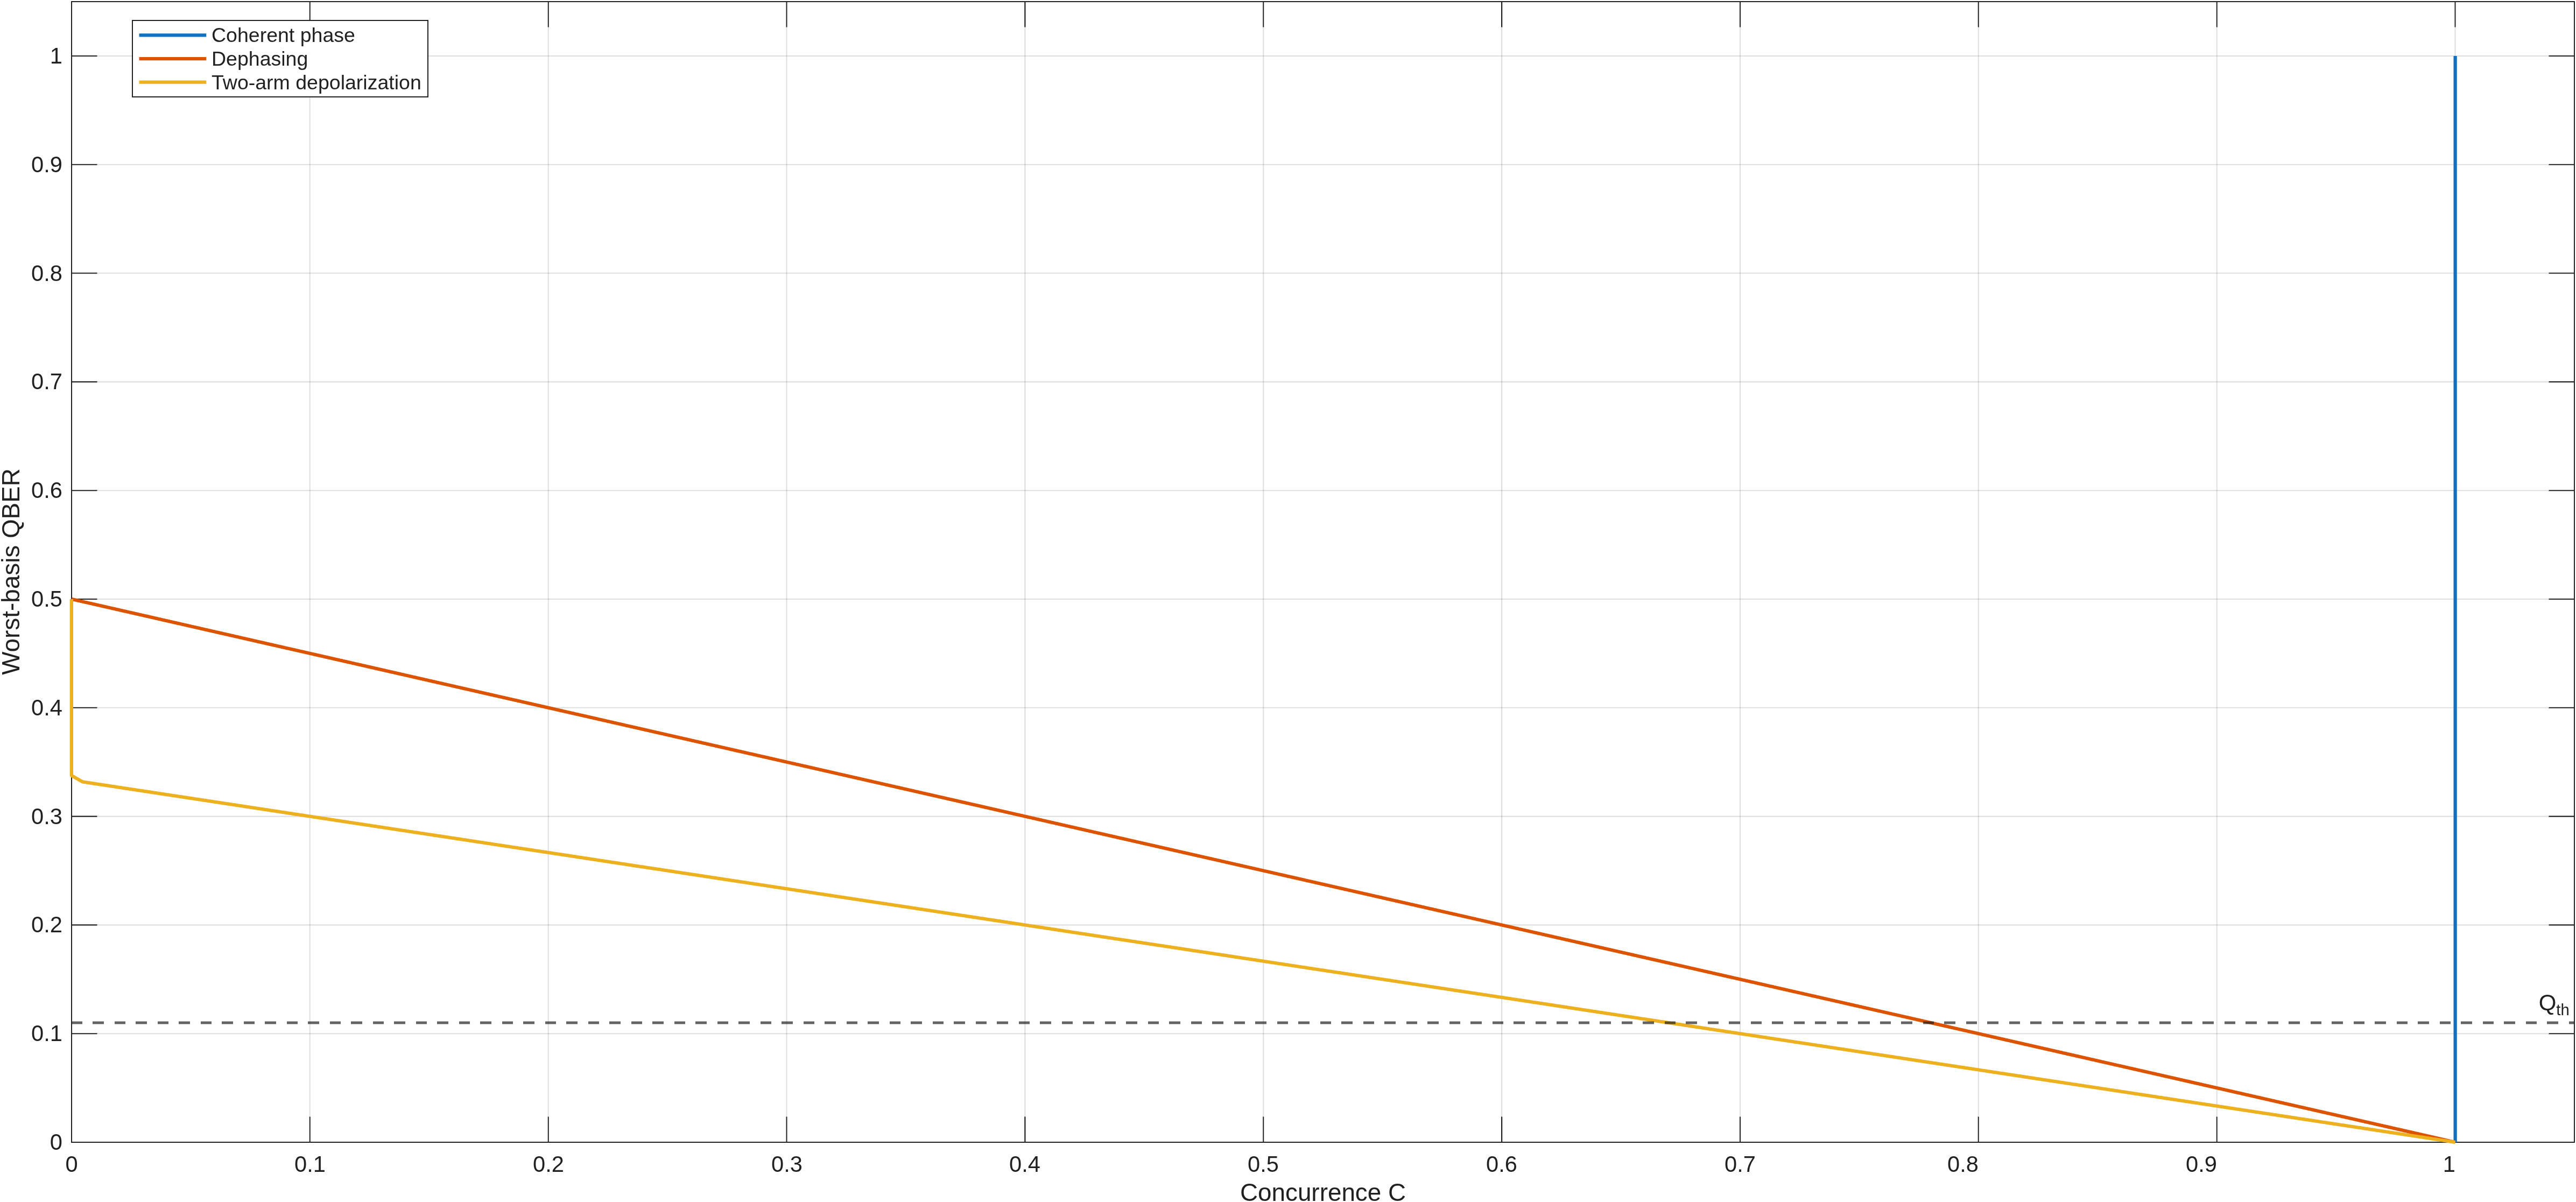
\includegraphics[
        width=0.98\textwidth
    ]{
        figures/experiment_1/concurrence_vs_qber.png
    }

    \caption{
        Worst-basis QBER as a function of concurrence for the three effective
        fiber models. The relation between entanglement and BBM92 performance
        depends on the physical degradation mechanism. Coherent phase evolution
        provides the limiting example in which \(C=1\) while the QBER varies.
    }

    \label{fig:exp1_concurrence_qber}

\end{figure}

The operating boundaries obtained from the three one-parameter models are

\begin{equation}
\boxed{
\theta_{\mathrm{th}}
\simeq
0.6761~\mathrm{rad},
\qquad
\mu_{\mathrm{th}}
=
0.780,
\qquad
p_{\mathrm{th}}
\simeq
0.1168.
}
\label{eq:exp1_boundaries_summary}
\end{equation}

These values parameterize different physical mechanisms and should therefore not
be interpreted as equivalent channel thresholds. Their common meaning is that
they identify where each model crosses the adopted BBM92 QBER criterion.

The experiment establishes the distinction used throughout the following
numerical analysis: purity, fidelity, and concurrence characterize different
properties of the distributed quantum state, whereas the BBM92 operating region
is determined directly from the measurement error rates. The subsequent
experiments extend this criterion from effective channel parameters to the
physical source and fiber parameters of the frequency-dependent propagation
model.